% !TeX spellcheck = it_IT
\section{Due esempi di corollari}

% --- Il teorema di Chow e Gulliver ---
\begin{frame}{Due corollari}{}
	\begin{block}{Corollario (Chow)}<1->
		Data una soluzione $C^2$ al problema, esiste $C$, \textbf{che dipende solo dal dato iniziale}, tale che ad ogni istante $t$:
		\begin{equation}
			\max_{x\in X_t} |x| - \min_{x\in X_t} |x| <C
		\end{equation}
	\end{block}
	\begin{block}{}<2->
		Se considero la soluzione riscalata, $\frac{X_t}{\max_{x\in X_t} |x|}$, per un flusso espansivo dove $\lim_{t\rightarrow T}\max_{x\in X_t} |x| = +\infty$, converge a una sfera 
	\end{block}
	\begin{block}{Corollario (Risa-Sinestrari)}<3->
		Non esistono soluzioni antiche espansive ($F<0$) che \textit{escono fuori da un punto} oltre alle sfere. 
	\end{block}
\end{frame}

\section{Cenni sulla parte originale della tesi}
% --- Frame: text and figure ---
\begin{frame}{Estensione a spazi a curvatura costante}{Idea}
	\begin{columns}
		% First column
		\column{.5\textwidth}
		Il risultato di Chow e Gulliver si estende al caso in cui lo spazio ambiente è $\mathbb{H}^{n+1}$ o $S^{n+1}$. 
		\begin{itemize}
			\item<1-> L'equazione continua ad essere parabolica anche negli spazi a curvatura costante
			\item<2-> Introduciamo una notazione che consente di impostare il problema
			\item<3-> La dimostrazione di Chow-Gulliver può essere estesa
		\end{itemize}
		% Second column
		\column{.5\textwidth}
		\begin{figure}
			\begin{center}
				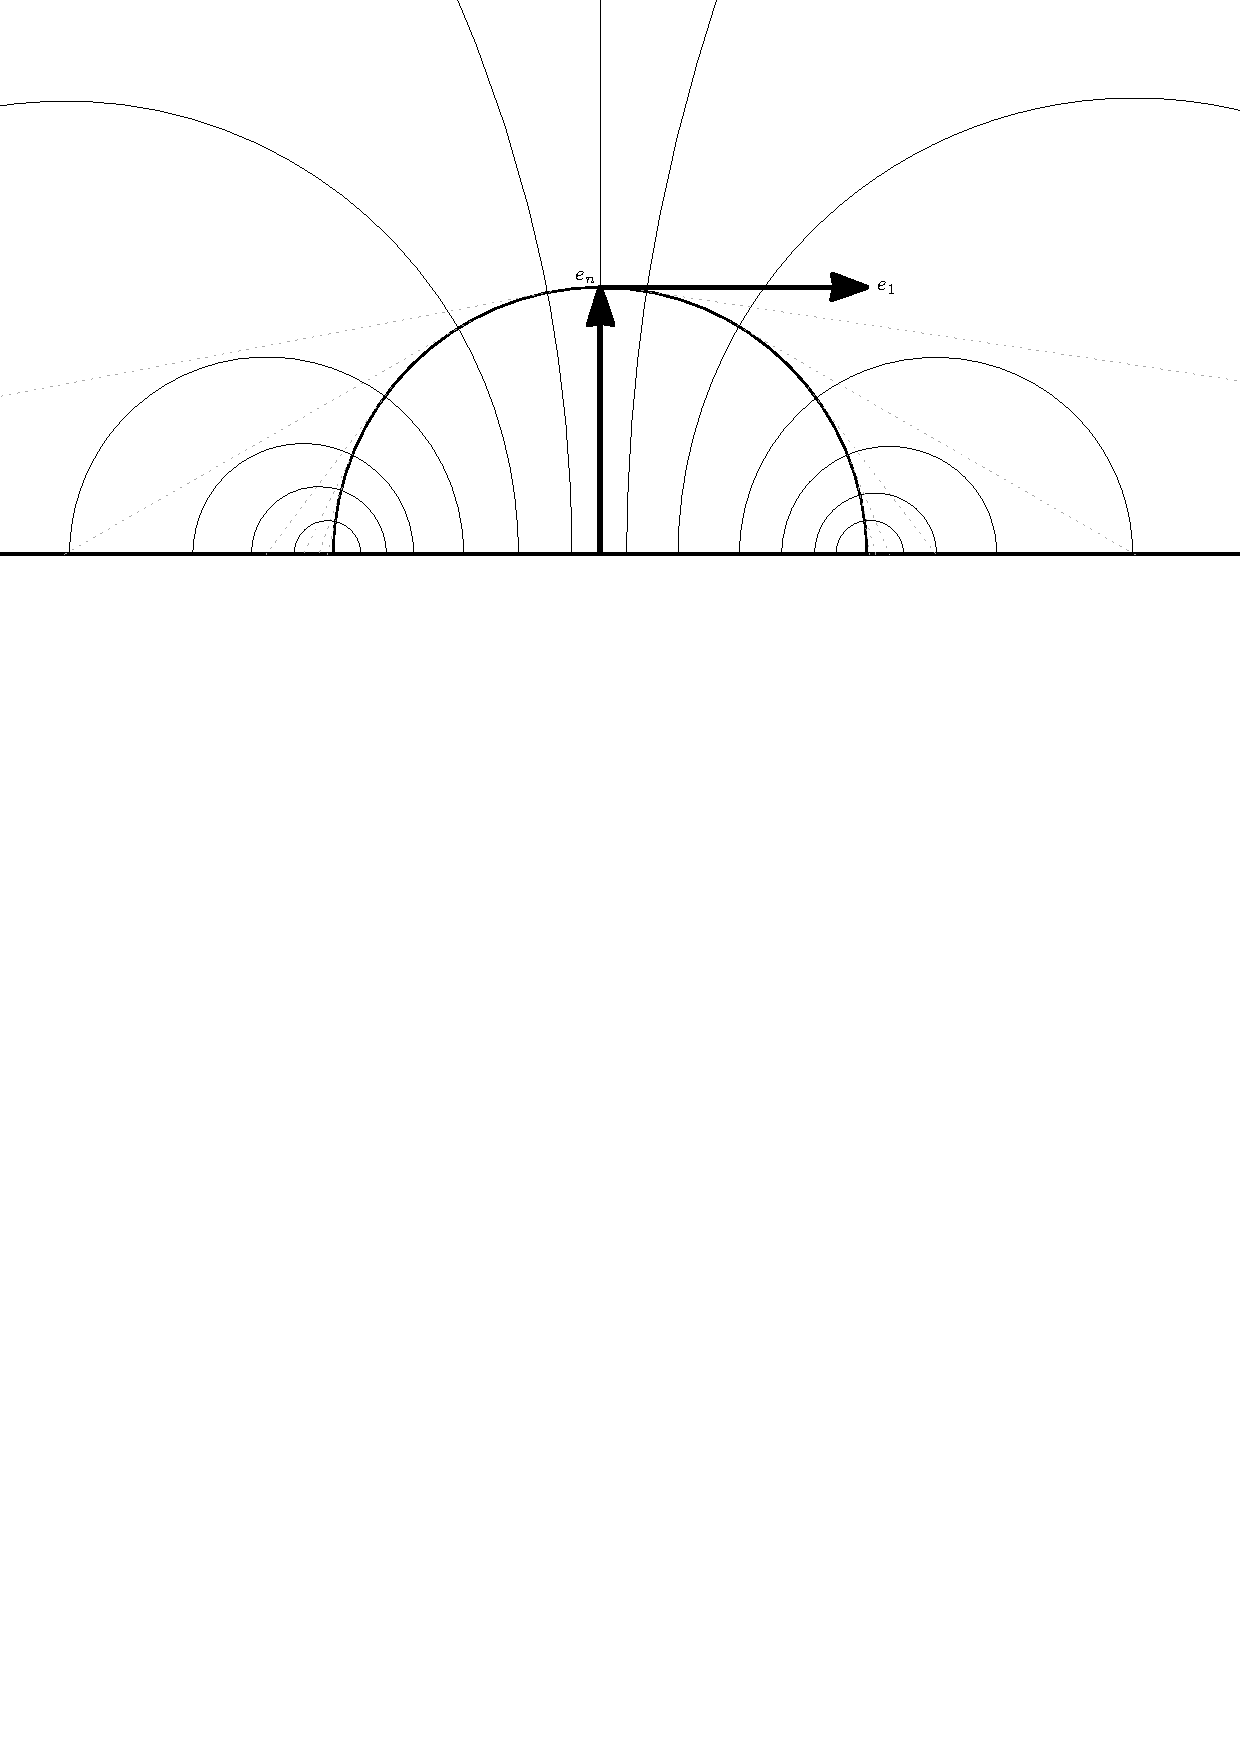
\includegraphics[width=\textwidth]{5b_moving_planes_hyperbolic}
				\caption{Iperpiani totalmente geodetici perpendicolari a una data geodetica in $\mathbb{H}^2$}
			\end{center}
		\end{figure}
	\end{columns}
\end{frame}

% --- Frame: text and figure ---
\begin{frame}{Estensione a spazi a curvatura costante}{Differenze con il caso euclideo}
	\begin{columns}
		% First column
		\column{.5\textwidth}
		\begin{itemize}
			\item<1-> Iperpiani sostituiti da superfici totalmente geodetiche
			\item<2-> Anche dimostrare che delle riflessioni esistono non è più banale
			\item<3-> Non è più ben definito un concetto di parallelismo tra gli iperpiani 
			\begin{itemize}
				\item Nel metodo consideriamo quelli ortogonali a una geodetica, ma non restano equidistanti in tutti i punti
			\end{itemize}
			\item<4-> Il trasporto parallelo non è banale
		\end{itemize}
		% Second column
		\column{.5\textwidth}
		\begin{figure}
			\begin{center}
				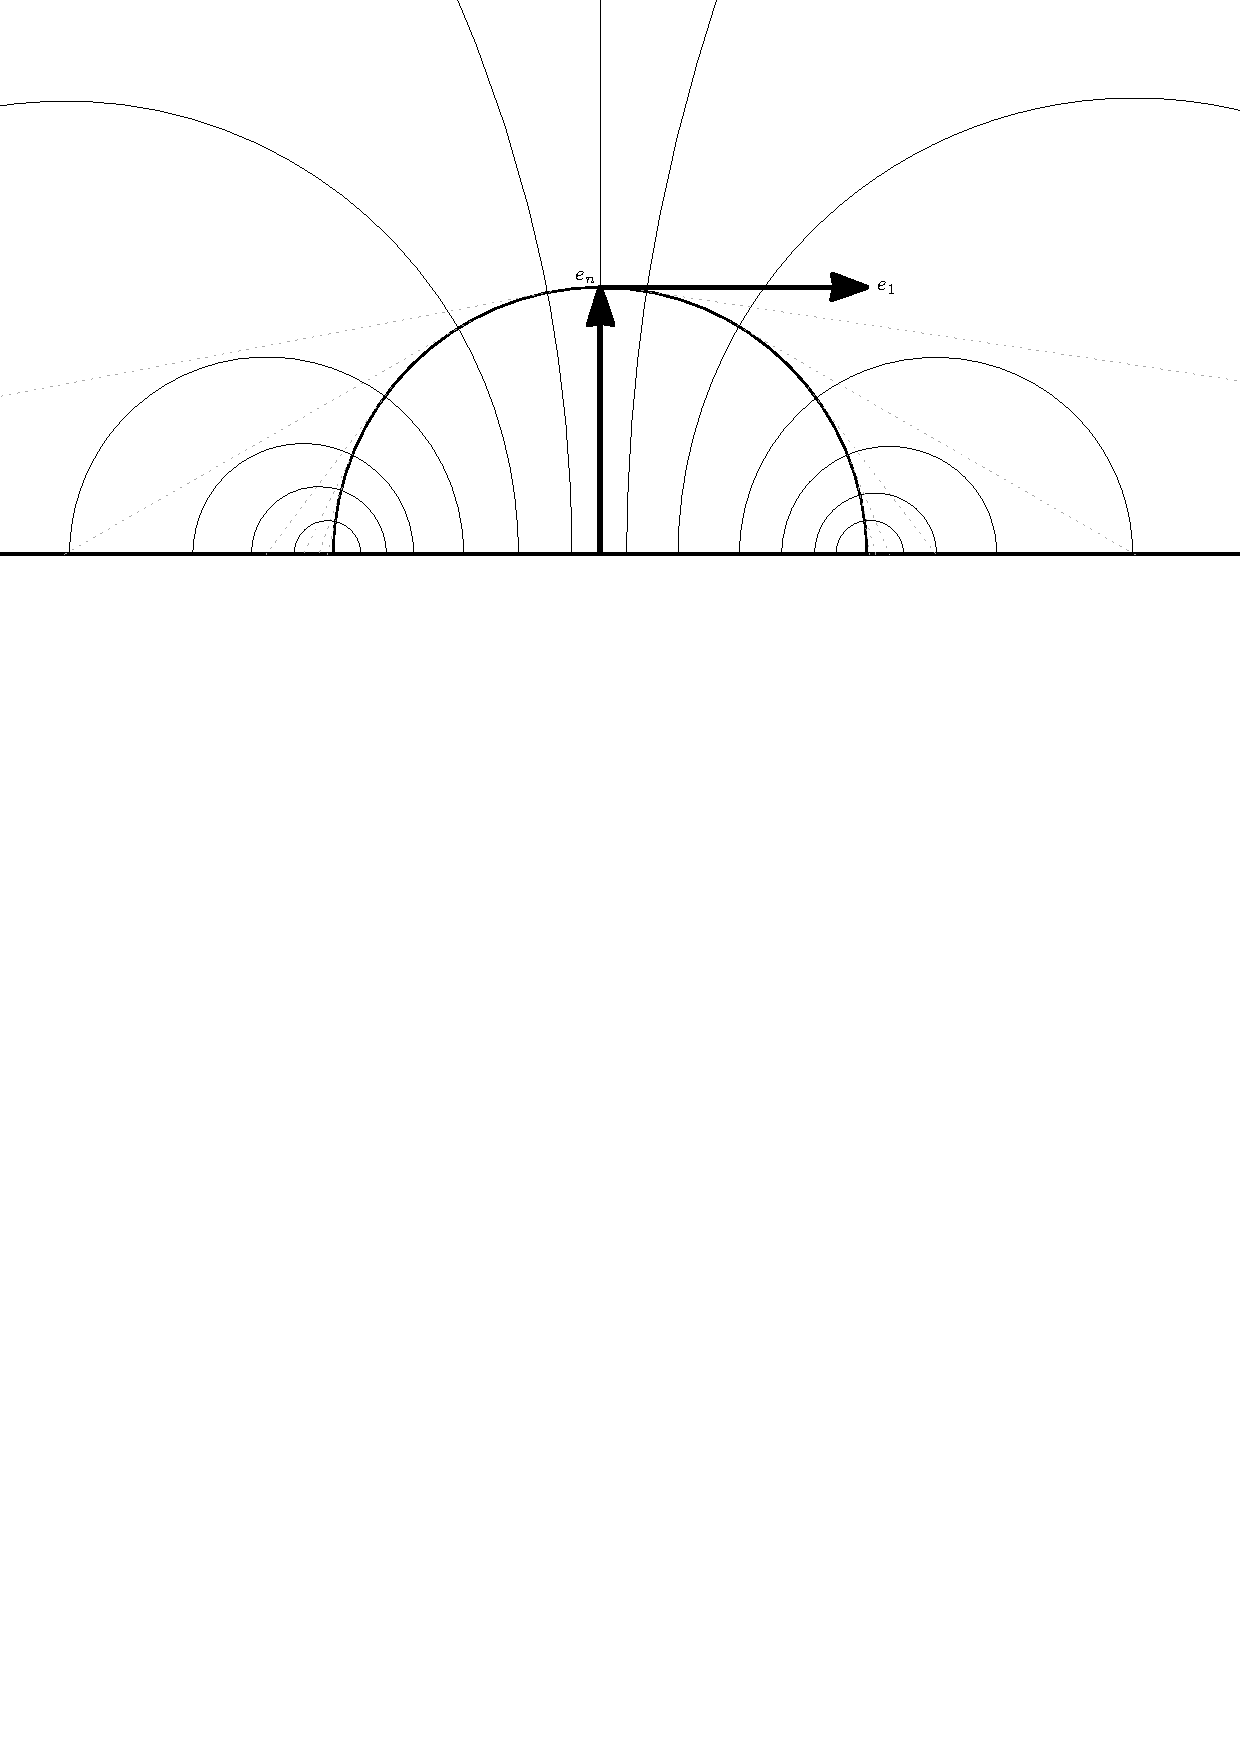
\includegraphics[width=\textwidth]{5b_moving_planes_hyperbolic}
				\caption{Iperpiani totalmente geodetici perpendicolari a una data geodetica in $\mathbb{H}^2$}
			\end{center}
		\end{figure}
	\end{columns}
\end{frame}


% --- Frame: text and figure ---
\begin{frame}{Estensione a spazi a curvatura costante}{Corollari}
	Alcuni corollari continuano a valere, ad esempio resta vero che 
	\begin{block}{Corollario}
		Non esistono soluzioni antiche espansive ($F<0$) che \textit{escono fuori da un punto} oltre alle sfere (intese come luogo dei punti equidistanti da un'origine). 
	\end{block}
\end{frame}


% --- Frame: text and figure ---
\begin{frame}{Estensione a spazi a curvatura costante}{Corollari}
	Alcuni corollari continuano a valere, ad esempio resta vero che 
	\begin{block}{Corollario}
		Non esistono soluzioni antiche espansive ($F<0$) che \textit{escono fuori da un punto} oltre alle sfere (intese come luogo dei punti equidistanti da un'origine). 
	\end{block}
	%Sulla sfera esiste anche una specie di risultato inverso di altri autori, dimostrato con altre tecniche di riflessione:
	%\begin{block}{Corollario}
		%Per una soluzione \textit{contrattiva} e \textit{convessa}, definita sul massimo intervallo possibile e dove il $\lim \sup$ della curvatura media è finita, allora il flusso è composto da sfere che si contraggono
	%\end{block}
\end{frame}



% --- Equazione di cui ci occupiamo ---
\begin{frame}{Flussi ad area e volume costante}{}
	\begin{block}{Flusso ad area/volume costante}
		\begin{align*}
			\frac{\partial X_t}{\partial t} = \left(-\frac{\sum_i \kappa_i(x)}{n}+\phi(t)\right) \nu
		\end{align*}
		consideriamo il flusso dove $F$ è la curvatura media $H$, e aggiungiamo un termine globale che lo rende a area/volume costante. Per conservare il volume: 
		\begin{align*}
			\phi(t) = \frac{\int_{X_t} H^2(x, t) \, d\mu}{\int_{X_t} H(x, t) \, d\mu}
		\end{align*}
	\end{block}
	\begin{block}{}<2->
		Il teorema di Chow e Gulliver si estende anche a questa classe di flussi
	\end{block}
	\begin{block}{}<3->
		Usando il metodo è possibile dimostrare che il flusso non esce fuori da un compatto
	\end{block}
\end{frame}

